\chapter{Intro to Sets}

\section{Examples, Notation \& properties}
One of the most fundamental structures you will come across during this course is a \emph{set}. Let's define what a set is:

\begin{dfn}[label={def:set}]{Set}{dfnSet}
    A \emph{set} is a collection of items.\\
    Examples:
    \begin{itemize}
        \item A = Students in a class
        \item B = \{1,3,4,7\} - Note the curly brackets, this is how you write out a set
        \item $\Z$ = Integers
    \end{itemize}

    \textbf{Note} - Order and repetition doesn't matter, so the set $$\{1,3,4,7\} = \{1,7,3,4\} = \{1,3,7,3,1,4,7\}$$
\end{dfn}

\begin{dfn}[label={def:elements}]{Elements}{dfnElements}
    An \emph{element} is an item inside a set. An item $x$ is said to be an element of set $X$ and is denoted as $x \in X$\\
    Examples:
    \begin{itemize}
        \item A student names John is an \emph{element} of set A above
        \item $ 4 \in $ set B
        \item $ 1 \in \Z$ but $\pi \notin \Z$ - this is read as $\pi$ is \emph{not} in $\Z$.
    \end{itemize}
\end{dfn}

\begin{dfn}[label={def:subset}]{Subsets}{dfnSubsets}
    A set $A$ is a subset of set $X$ if every element of $A$ is also an element of $X$. This is denoted as $A \subseteq X$. In this situation $X$ is called the \emph{superset} of $A$. \\
    Examples:
    \begin{itemize}
        \item $\{1,3\} \subseteq \{1,3,4,7\}$
        \item $\{1,3,4,2\}$ is not a subset of $\{1,3,4,7\}$ since the latter set doesn't contain 2. This is denoted as $\{1,3,4,2\} \nsubseteq \{1,3,4,7\}$
    \end{itemize}
\end{dfn}

\section{Set-Roster vs Set-Buider notation}

Sets are incredibly useful, but we need to be able to write them down if we're going to be using them going forward. We'll now look at two different ways of denoting a set.

\subsection*{Set-Roster}
The notation we've been using so far, using the \{\} with elements listed inside, is called \emph{set-roster} notation. One of the biggest issues with this notation is that we might have an incredibly large set - we don't want to have to write out each element.

One way aroumd this is, if we have a pattern to the elements, we can use elipses to indicate the pattern continues. For example
$$\{0,2,4,6,\dots\}$$
This denotes the set of all positibe even integers, starting from 0.
$$\{\dots,-6,-4,-2,0,2,4,6,\dots\}$$
This now indicates all the even integers - positive \textbf{and} negative.

This is very useful, but only if there is a clearly recognisable pattern that can be seen from only a few elements. If the pattern is not obvious, we need a different way of writing this.

\subsection*{Set-Builder}
\emph{Set-builder} notation allows us to specify much more complex patterns/restrictions for the elements of a set. The general for is
$$\{\underbrace{x}_{\text{variable }} \underbrace{|}_{\text{ read as 'such that' }} \underbrace{P(x)}_{\text{ Property is True}}\}$$
The way to read this notation is ``the set of all $x$ such that $x$ has property $P(x)$".

Let's look at some examples
\begin{exmpl}[label={exmpl:evenints}]{Set of Even Integers}{xmpEvenInts}
    Say we would like the set of all even integers. We can define this by saying we want the set of all $x$ such that $x$ is the product of 2 and some other integer. Using set-builder notation we can write this as
    $$\{x | x = 2k, k \in \Z\}$$
    This allows us to select for any even integer. For example, 6 is in this set because $6 = 2 \times 3$ and $3 \in \Z$.
\end{exmpl}

\begin{exmpl}[label={exmpl:intsqrt}]{Set of Integer Squares}{xmpintsqrt}
    Say we would like the set of all numbers whose square root is an integer. Another way of saying this is the set of all numbers that you get when you square each member of the integers. We can write this as
    $$\{x | x = k^2, k \in \Z\}$$
    The number 9 would be in this set since $9 = 3^2$ and $3 \in \Z$. The number 6 would \emph{not} be in this set since there is no integer (no element of $\Z$) that gives you six when you square it.
\end{exmpl}

\section{The Empty Set \& Vacuous Truth}
So far we've talked about sets as a collection of items, these items can be random or they can follow some kind of pattern. The very next question you should be asking yourself is - \emph{what about a set with nothing in it?} This is where we define the \emph{empty set}.

\begin{dfn}[label={def:emptyset}]{The Empty Set}{dfnemptyset}
    The \emph{empty set} is the set defined by having no elements. This can be written in one of two ways
    $$\{\} \quad \text{or} \quad \emptyset$$
\end{dfn}

The empty set is a strange concept to get your head around at first, but it allows us to really examine the properties of sets.

For example, let's consider $\{\emptyset\}$. At first glance you might consider this set to be empty, but that would be incorrect. The empty set, $\emptyset$, is empty, but this set has an element, that element is $\emptyset$. You might find it useful to consider sets to be boxes - the empty set is a box with nothing in it, this set is a box with \emph{another} empty box inside it.

Let's try another, is $\emptyset \subseteq \{1,2,3\}$? Let's remind ourselves of \cref{def:subset} - \emph{A set A is a subset of set X if every element of A is also an element of X}. While it may seem counter-inuitive, the empty set is indeed a subset of $\{1,2,3\}$ - because $\emptyset$ has no elements, then it follows that any element of $\emptyset$ is also in $\{1,2,3\}$ - in fact this is true for \emph{any} set, $\emptyset$ is always a subset of any other set.

This is a case of what we call \emph{vacuous truth}. This is the situation where a statement can be true and the same time as the opposing statement also being true. In this example, we can say both that \emph{every} element that is in $\emptyset$ is in $\{1,2,3\}$, and that \emph{none} of the elements in $\emptyset$ are in $\{1,2,3\}$.

\section{Cartesian Product of Two Sets}
We've looked at a few different kind of sets up to now, so we're going to move onto looking at a new kind of \emph{elememt} of sets - an \emph{ordered pair}.

\begin{dfn}[label={def:orderedpairs}]{Ordered Pairs}{dfnorderedpairs}
    An \emph{ordered pair} is an object made up of two elements, where the \emph{order matters}
    $$(a,b) \neq (b,a)$$
    $$(a,b) = (c,d) \implies a = c\  \& \ b=d$$
    These elements can also come from entirely different sets.
\end{dfn}

Now that we have a definition for ordered pairs, what could we say about the set whose elements were all ordered pairs? This is known as the \emph{Cartesian Product} of two sets.

\begin{dfn}[label={def:cartprod}]{Cartesian Product of Two Sets}{dfncartprod}
    The \emph{Cartesian Product} of two sets, denoted $A \times B$, is the set of all ordered pairs $(a,b)$ where $a \in A$ and $b \in B$
\end{dfn}

\begin{exmpl}[label={exmpl: cartplane}]{The Cartesian Plane}{xmpcartplane}
    A well known example of a Cartesian product is the Cartesian plane (a.k.a the $xy$-plane). This plane is product of the set of real numbers, $\R$, with itself
    $$plane_c = \{(x,y) | x,y \in \R\}$$
\end{exmpl}

\newpage

\begin{figure}[ht]
    \label{fig:pointOnPlane}
    \begin{center}
        \begin{tikzpicture}
            \begin{axis}[xmin=-3,
                    xmax=3,
                    ymin=-2,
                    ymax=2,
                    axis lines = middle,
                    xlabel=$x$,
                    ylabel=$y$,
                    title={The Cartesian Plane}]
                \node[label={$(2,1) \in \R \times \R$},circle,fill,inner sep=2pt] at (axis cs:2,1) {};
            \end{axis}
        \end{tikzpicture}
    \end{center}
    \caption{A point on the Cartesian Plane}
\end{figure}

\vspace{1cm}

\begin{exmpl}[label={exmpl: cart2sets}]{The Cartesian product of Two Sets}{xmpcart2sets}
    Here's an exmaple of the Cartesian product of two smaller sets, $A,b$ where $A = \{a,b\}$ and $B = \{0,1\}$. So we have
    $$A \times B = \{(a,0), (a,1),(b,0),(b,1) \}$$
\end{exmpl}

\section{Relations Between Two Sets}
We come across relations in mathematics all the time, one very familiar relation is the $\leq$ relation. This is a relation between two numbers that tells us if the first is smaller (or equal to) the second, e.g. $2 \leq 5$. Some relations, such as $\leq$, are dependant on order, e.g. we know that $5 \not\leq 2$.

We can also define relations between sets. Let's look at an example to begin with

\begin{exmpl}[label={exmpl: relation2sets}]{Visual Relation Between 2 Sets}{xmprelation2sets}
    Imagine we had a set of humans and set of pets, we could define a relation called 'ownership' where a human is related to a pet if the human owns that pet. We could then draw a visual of this with arros pointing from humans to the pets they own.
    \begin{center}
        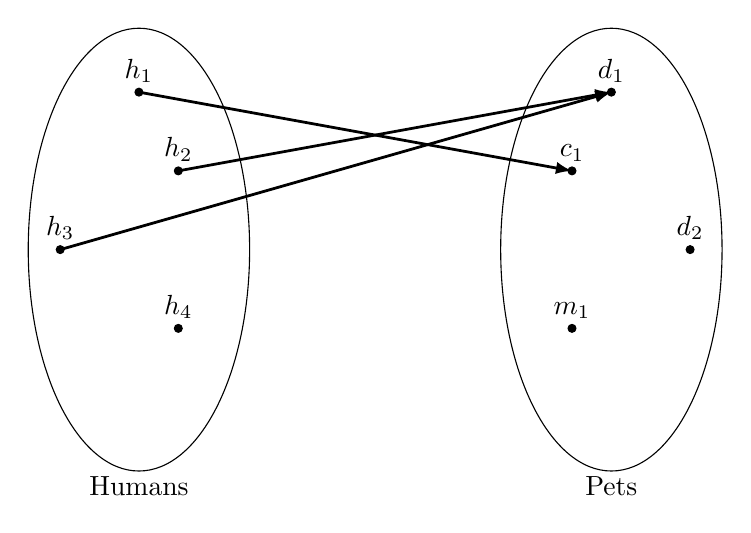
\begin{tikzpicture}
            \draw(2,0) ellipse (40pt and 80pt);
            \draw node at (2,-3){Humans};
            \draw(8,0) ellipse (40pt and 80pt);
            \draw node at (8,-3){Pets};

            %Nodes
            \filldraw (2,2) circle (0.05cm) node[anchor=south]{$h_1$};
            \filldraw (2.5,1) circle (0.05cm) node[anchor=south]{$h_2$};
            \filldraw (1,0) circle (0.05cm) node[anchor=south]{$h_3$};
            \filldraw (2.5,-1) circle (0.05cm) node[anchor=south]{$h_4$};
            \filldraw (8,2) circle (0.05cm) node[anchor=south]{$d_1$};
            \filldraw (7.5,1) circle (0.05cm) node[anchor=south]{$c_1$};
            \filldraw (9,0) circle (0.05cm) node[anchor=south]{$d_2$};
            \filldraw (7.5,-1) circle (0.05cm) node[anchor=south]{$m_1$};

            %Lines
            \draw[->, >=latex, line width=1pt] (2,2) -- (7.5,1);
            \draw[->, >=latex, line width=1pt] (2.5,1) -- (8,2);
            \draw[->, >=latex, line width=1pt] (1,0) -- (8,2);
        \end{tikzpicture}
    \end{center}
    This defines ordered pairs with the human as the first entry, e.g. $(h_1, c_1)$ means that Human 1 owns Cat 1.
\end{exmpl}

This example gives a good intuitive understanding of what a relation is, but it doesn't count as a formal definition of a relation between two sets. We can define a relation as below

\begin{dfn}[label={def:relation2sets}]{Relation Between Two Sets}{dfnrelation2sets}
    A \emph{relation}, $R$, between the sets $A$ and $B$ is a subset of $A \times B$.
    $$R = \{(a,b) | (a,b) \in A \times B\}$$
\end{dfn}

We will look more closely at relations in the future, but for now this should give you a good foundational understanding of sets, how they can relate to each other, and how those relations can create sets themselves.

Next, we will be looking at how sets and functions are related.